\chapter{Signal Propagation: Travelling and Standing Waves}\label{ch:b1:wave-propagation}

Pluck a guitar string and a whole hall hears a note; hold a finger
lightly at its midpoint and the note jumps an octave. Stand between two
loudspeakers playing the same tone and, walking slowly, you cross spots
of near silence every few decimeters. Light from two pinholes paints
stripes on a screen. Nothing is carried from one place to another in any
of these --- no air, no string, no glass travels --- yet something
propagates: a \emph{\omterm{def:b1:wave-propagation:signal}{signal}}. This chapter describes how a \omterm{def:b1:wave-propagation:signal}{signal} moves,
what a sinusoidal wave is, and what happens when two waves meet: the
mathematics of superposition, interference, and \omterm{thm:b1:wave-propagation:standing}{standing waves}, which
every later wave chapter --- acoustics, optics, and quantum physics ---
will reuse.

\begin{omfigure}
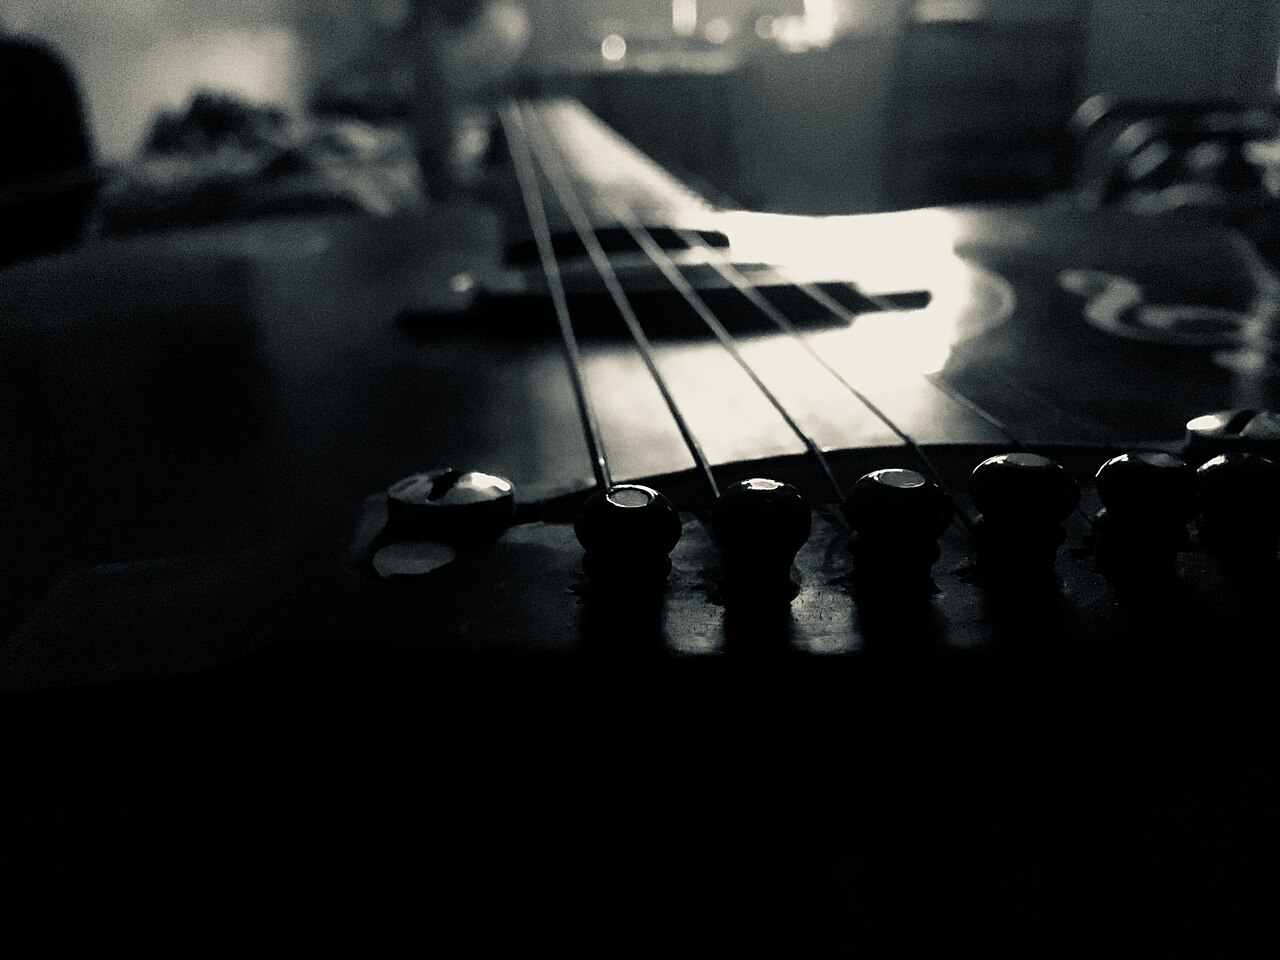
\includegraphics[width=0.55\linewidth]{images/book3/guitar-closeup.jpg}

{\small Six strings, six fundamental frequencies: each is a \omterm{thm:b1:wave-propagation:standing}{standing wave} fixed at the nut and the bridge, and the fingers shorten it to raise the pitch.}
\end{omfigure}

\section{Signals}

\begin{definition}[Signal; sinusoidal signal]\label{def:b1:wave-propagation:signal}
\index{signal}\index{sinusoidal signal}\index{amplitude}\index{phase}\index{angular frequency}
A \emph{signal} is a \omterm{def:b1:units-dimensions:unit}{physical quantity} that varies in time and carries
information: the acoustic overpressure at a microphone, the voltage at
an antenna, the transverse displacement of a point of a string. The
\emph{sinusoidal signal}
\[
s(t) = A\cos(\omega t + \varphi)
\]
has \emph{amplitude} $A > 0$, \emph{angular frequency} $\omega$
(\unit{rad/s}), \emph{frequency} $f = \omega/2\pi$, \emph{period}
$T = 1/f$ and \emph{initial phase} $\varphi$; $\omega t + \varphi$ is
its \emph{phase} at time $t$.
\end{definition}

\begin{remark}[Spectrum]\label{rem:b1:wave-propagation:spectrum}
\index{spectrum!of a signal}\index{harmonic}
Any periodic \omterm{def:b1:wave-propagation:signal}{signal} of period $T$ is a sum of sinusoids of frequencies
$f_1 = 1/T$ (the \emph{fundamental}) and its multiples $nf_1$ (the
\emph{harmonics}); the list of their \omterm{def:b1:wave-propagation:signal}{amplitudes} is the \omterm{def:b1:wave-propagation:signal}{signal}'s
\emph{spectrum}. A flute and a violin playing the same note share the
fundamental and differ in the spectrum --- that is timbre. The
decomposition (Fourier's) is stated and used in
\cref{ch:b1:filters-transfer-functions}; here it matters because
sinusoids propagate simply, and whatever holds for each sinusoid holds,
by addition, for any \omterm{def:b1:wave-propagation:signal}{signal}.
\end{remark}

\begin{proposition}[Beats]\label{prop:b1:wave-propagation:beats}
\index{beats}
The sum of two sinusoids of equal \omterm{def:b1:wave-propagation:signal}{amplitude} and close frequencies
$f_1 > f_2$,
\[
A\cos(2\pi f_1 t) + A\cos(2\pi f_2 t)
= 2A\cos\!\big(2\pi\tfrac{f_1 - f_2}{2}\,t\big)\cos\!\big(2\pi\tfrac{f_1 + f_2}{2}\,t\big),
\]
is a sinusoid at the mean frequency whose \omterm{def:b1:wave-propagation:signal}{amplitude}
$\abs{2A\cos(\pi(f_1 - f_2)t)}$ swells and fades at the \emph{beat
frequency} $f_1 - f_2$.
\end{proposition}

\begin{proof}
$\cos a + \cos b = 2\cos\frac{a - b}{2}\cos\frac{a + b}{2}$. The slow
factor vanishes twice per period $2/(f_1 - f_2)$ of its own, so the
envelope $\abs{\cdot}$ has frequency $f_1 - f_2$.
\end{proof}

\begin{omfigure}
\begin{tikzpicture}
\begin{axis}[omaxis, axis x line=bottom, width=11.5cm, height=4.6cm, xlabel={$t$ (\unit{s})},
    ylabel={$s$}, xmin=0, xmax=1, ymin=-2.3, ymax=2.3, ytick={-2,0,2},
    yticklabels={$-2A$,$0$,$2A$}, xtick={0,0.25,0.5,0.75,1}]
  \addplot[omDef, thick, domain=0:1, samples=700] {cos(deg(2*pi*22*x)) + cos(deg(2*pi*20*x))};
  \addplot[omThm, thick, dashed, domain=0:1, samples=200] {2*cos(deg(2*pi*1*x))};
  \addplot[omThm, thick, dashed, domain=0:1, samples=200] {-2*cos(deg(2*pi*1*x))};
\end{axis}
\end{tikzpicture}

{\small Beats between \qty{22}{Hz} and \qty{20}{Hz}: a \qty{21}{Hz}
oscillation whose envelope (dashed) beats twice per second --- the
difference of the frequencies.}
\end{omfigure}

\begin{example}[Tuning by ear]\label{ex:b1:wave-propagation:tuning}
A tuning fork at \qty{440}{Hz} and a string at \qty{443}{Hz} sounded
together throb three times a second; tightening the string slows the
throb, and when it stops the string is in tune. The ear hears the mean
frequency (\qty{441.5}{Hz}) as the pitch and the \qty{3}{Hz} envelope as
loudness wobbling: beats make a frequency difference of less than one
percent audible.
\end{example}

\section{Travelling waves}

\begin{definition}[Travelling wave, celerity]\label{def:b1:wave-propagation:travelling}
\index{travelling wave}\index{celerity}\index{non-dispersive medium}
A \omterm{def:b1:wave-propagation:signal}{signal} $s(x, t)$ defined along an axis is a \emph{travelling wave}
moving in the $+x$ direction at \emph{celerity} $c$ if
\[
s(x, t) = f\!\left(t - \frac{x}{c}\right) = F(x - ct)
\]
for some function $f$ (or $F$): the shape is carried along unchanged,
shifted by $c\,\Delta t$ in time $\Delta t$. A wave moving toward $-x$ is
$g(t + x/c)$. A medium in which every shape propagates undeformed at
the same $c$ is \emph{non-dispersive}.
\end{definition}

\begin{proposition}[Delay]\label{prop:b1:wave-propagation:delay}
The \omterm{def:b1:wave-propagation:signal}{signal} received at $x_2$ is the \omterm{def:b1:wave-propagation:signal}{signal} emitted at $x_1 < x_2$,
delayed by $\tau = (x_2 - x_1)/c$: $s(x_2, t) = s(x_1, t - \tau)$.
\end{proposition}

\begin{proof}
$s(x_2, t) = f(t - x_2/c) = f\big((t - \tau) - x_1/c\big) = s(x_1, t - \tau)$.
\end{proof}

\begin{example}[Celerities]\label{ex:b1:wave-propagation:celerities}
Sound in air, \qty{340}{m/s}: thunder \qty{3}{s} after the flash puts
the strike \qty{1}{km} away. Sound in water, \qty{1500}{m/s}; in steel,
\qty{5000}{m/s}. Transverse waves on a string of tension $F$ and mass
per unit length $\mu$: $c = \sqrt{F/\mu}$, as dimensional analysis
predicted (\cref{exo:b1:units-dimensions:5}) --- \qty{140}{m/s} for a
guitar string. Light in vacuum, $c = \qty{3.00e8}{m/s}$; in glass,
$c/n$. The \omterm{def:b1:wave-propagation:travelling}{celerity} is a property of the medium, not of the source: a
whisper and a shout arrive together.
\end{example}

\begin{proposition}[Sinusoidal travelling wave]\label{prop:b1:wave-propagation:sinusoidal}
\index{wavelength}\index{wavenumber}\index{phase velocity}\index{double periodicity}
A sinusoidal source $s(0, t) = A\cos(\omega t)$ launches
\[
s(x, t) = A\cos\!\big(\omega(t - x/c)\big) = A\cos(\omega t - kx),
\qquad k = \frac{\omega}{c} = \frac{2\pi}{\lambda},
\qquad \lambda = cT = \frac{c}{f}.
\]
The wave is periodic in time (period $T$) and in space (period the
\emph{wavelength} $\lambda$); $k$ is the \emph{wavenumber}; two points
a distance $d$ apart oscillate with a \omterm{def:b1:wave-propagation:signal}{phase} difference
$\Delta\varphi = 2\pi d/\lambda = kd$ --- in \omterm{def:b1:wave-propagation:signal}{phase} if $d = n\lambda$, in
opposite \omterm{def:b1:wave-propagation:signal}{phase} if $d = (n + \tfrac12)\lambda$. The speed at which a
crest moves, $v_\varphi = \omega/k$, is the \emph{\omterm{prop:b1:wave-propagation:sinusoidal}{phase velocity}};
here $v_\varphi = c$.
\end{proposition}

\begin{proof}
Substitute $f(u) = A\cos(\omega u)$ into $f(t - x/c)$. At fixed $x$ the
\omterm{def:b1:wave-propagation:signal}{signal} repeats after $T = 2\pi/\omega$; at fixed $t$ it repeats after
$\lambda$ with $k\lambda = 2\pi$. Two points $x_1$, $x_2 = x_1 + d$: the
\omterm{def:b1:wave-propagation:signal}{phases} differ by $kd$. A crest ($\omega t - kx = \text{const}$) moves at
$\dd x/\dd t = \omega/k$.
\end{proof}

\begin{omfigure}
\begin{tikzpicture}
\begin{axis}[omaxis, width=7.2cm, height=4.2cm, xlabel={$x$}, ylabel={$s(x, t_0)$},
    xmin=0, xmax=6.5, ymin=-1.4, ymax=1.6, ytick={-1,0,1}, yticklabels={$-A$,$0$,$A$},
    xtick={0,2,4,6}, xticklabels={$0$,$\lambda$,$2\lambda$,$3\lambda$}]
  \addplot[omDef, thick, domain=0:6.5, samples=200] {cos(deg(pi*x))};
  \draw[Stealth-Stealth, omThm] (axis cs:2,1.2) -- (axis cs:4,1.2) node[midway, above, font=\footnotesize] {$\lambda$};
  \draw[-Stealth, omExo, thick] (axis cs:4.7,1.2) -- (axis cs:5.7,1.2) node[midway, above, font=\footnotesize] {$c$};
\end{axis}
\end{tikzpicture}\qquad
\begin{tikzpicture}
\begin{axis}[omaxis, width=7.2cm, height=4.2cm, xlabel={$t$}, ylabel={$s(x_0, t)$},
    xmin=0, xmax=6.5, ymin=-1.4, ymax=1.6, ytick={-1,0,1}, yticklabels={$-A$,$0$,$A$},
    xtick={0,2,4,6}, xticklabels={$0$,$T$,$2T$,$3T$}]
  \addplot[omDef, thick, domain=0:6.5, samples=200] {cos(deg(pi*x))};
  \draw[Stealth-Stealth, omThm] (axis cs:2,1.2) -- (axis cs:4,1.2) node[midway, above, font=\footnotesize] {$T$};
\end{axis}
\end{tikzpicture}

{\small The \omterm{prop:b1:wave-propagation:sinusoidal}{double periodicity} of a sinusoidal \omterm{def:b1:wave-propagation:travelling}{travelling wave}: a
snapshot at fixed time repeats every wavelength $\lambda$ and slides at
speed $c$; the \omterm{def:b1:wave-propagation:signal}{signal} at a fixed point repeats every period $T$, with
$\lambda = cT$.}
\end{omfigure}

\begin{definition}[Dispersion]\label{def:b1:wave-propagation:dispersion}
\index{dispersive medium}
A medium is \emph{dispersive} when the \omterm{prop:b1:wave-propagation:sinusoidal}{phase velocity} depends on the
frequency. A non-sinusoidal \omterm{def:b1:wave-propagation:signal}{signal}, a sum of sinusoids, then deforms as
it travels, its components drifting apart. Sound in air and light in
vacuum are non-dispersive; light in glass (\cref{ch:b1:rays-reflection-refraction})
and waves on deep water are dispersive --- the long swell from a distant
storm arrives a day before the short chop.
\end{definition}

\section{Superposition and interference}

\begin{theorem}[Superposition]\label{thm:b1:wave-propagation:superposition}
\index{superposition principle}
In a linear medium, when several waves propagate together, the
resulting \omterm{def:b1:wave-propagation:signal}{signal} at each point and time is the sum of the \omterm{def:b1:wave-propagation:signal}{signals} each
wave would produce alone.
\end{theorem}
\admitted

\begin{remark}[Linearity]\label{rem:b1:wave-propagation:linearity}
Superposition is a statement about the equations of the medium (linear
in the \omterm{def:b1:wave-propagation:signal}{signal}), true as long as \omterm{def:b1:wave-propagation:signal}{amplitudes} stay small: sound below the
threshold of pain, light below laser-cutting intensities, a string
plucked gently. Two beams of light cross without disturbing each other;
two ripples pass through one another and emerge intact. What is
observed \emph{where they overlap} is the subject of interference.
\end{remark}

\begin{theorem}[Two sinusoidal signals of the same frequency]\label{thm:b1:wave-propagation:fresnel}
\index{interference}\index{Fresnel's formula}\index{constructive interference}\index{destructive interference}
At a point where two \omterm{def:b1:wave-propagation:signal}{sinusoidal signals} of the same frequency arrive,
$s_1 = A_1\cos(\omega t + \varphi_1)$ and $s_2 = A_2\cos(\omega t + \varphi_2)$,
the sum is a sinusoid of the same frequency whose \omterm{def:b1:wave-propagation:signal}{amplitude} satisfies
\[
A^2 = A_1^2 + A_2^2 + 2A_1A_2\cos\Delta\varphi,
\qquad \Delta\varphi = \varphi_2 - \varphi_1 .
\]
For waves whose intensity (power per unit area) is proportional to
$A^2$, the intensities obey \emph{Fresnel's formula}
\[
I = I_1 + I_2 + 2\sqrt{I_1 I_2}\,\cos\Delta\varphi .
\]
The interference is \emph{constructive} ($A = A_1 + A_2$) when
$\Delta\varphi = 2n\pi$, \emph{destructive} ($A = \abs{A_1 - A_2}$)
when $\Delta\varphi = (2n + 1)\pi$, $n \in \Z$.
\end{theorem}

\begin{proof}
Expand: $s_1 + s_2 = (A_1\cos\varphi_1 + A_2\cos\varphi_2)\cos\omega t -
(A_1\sin\varphi_1 + A_2\sin\varphi_2)\sin\omega t = X\cos\omega t -
Y\sin\omega t = A\cos(\omega t + \varphi)$ with $A^2 = X^2 + Y^2 =
A_1^2 + A_2^2 + 2A_1A_2(\cos\varphi_1\cos\varphi_2 + \sin\varphi_1\sin\varphi_2)$.
Geometrically: $A$ is the length of the sum of two vectors of lengths
$A_1$, $A_2$ making the angle $\Delta\varphi$ (the law of cosines).
\end{proof}

\begin{proposition}[Two sources in phase; path difference]\label{prop:b1:wave-propagation:pathdiff}
\index{path difference}
Two sources emitting in \omterm{def:b1:wave-propagation:signal}{phase} at wavelength $\lambda$, at distances
$d_1$ and $d_2$ from a point $M$, arrive at $M$ with
$\Delta\varphi = 2\pi\,\delta/\lambda$, where $\delta = d_2 - d_1$ is the
\emph{\omterm{prop:b1:wave-propagation:pathdiff}{path difference}}. Interference at $M$ is constructive if
$\delta = n\lambda$, destructive if $\delta = (n + \tfrac12)\lambda$.
\end{proposition}

\begin{proof}
Each wave arrives with the \omterm{def:b1:wave-propagation:signal}{phase} lag $kd_i = 2\pi d_i/\lambda$ of its
journey (\cref{prop:b1:wave-propagation:sinusoidal}); the difference is
$2\pi(d_2 - d_1)/\lambda$. Apply \cref{thm:b1:wave-propagation:fresnel}.
\end{proof}

\begin{example}[Two loudspeakers]\label{ex:b1:wave-propagation:speakers}
Two speakers \qty{2.0}{m} apart play the same \qty{850}{Hz} tone in
\omterm{def:b1:wave-propagation:signal}{phase} ($\lambda = \qty{0.40}{m}$). On the perpendicular bisector
$\delta = 0$: loud everywhere. Along the segment joining them, $\delta$
changes by $2\lambda$ per wavelength of displacement, so quiet spots
($\delta = \pm\lambda/2, \pm 3\lambda/2, \dots$) sit every
$\lambda/2 = \qty{20}{cm}$ --- a \omterm{thm:b1:wave-propagation:standing}{standing wave}, the subject of the next
section. Move one speaker's wire so it plays in opposite \omterm{def:b1:wave-propagation:signal}{phase}, and loud
and quiet exchange places.
\end{example}

\begin{example}[Young's holes]\label{ex:b1:wave-propagation:young}
\index{Young's holes}\index{fringe spacing}\index{optical path}
Two pinholes $S_1$, $S_2$ a distance $a$ apart, lit by one
monochromatic source (so that they emit in \omterm{def:b1:wave-propagation:signal}{phase}), send light to a
screen at distance $D \gg a$. At a point of the screen at height $x$
from the axis, the \omterm{prop:b1:wave-propagation:pathdiff}{path difference} is
\[
\delta = S_2M - S_1M \approx \frac{a\,x}{D}
\]
(for $x \ll D$: $S_{1,2}M = \sqrt{D^2 + (x \mp a/2)^2} \approx D +
(x \mp a/2)^2/2D$, and subtract). Bright fringes at $x = n\lambda D/a$:
the \emph{\omterm{ex:b1:wave-propagation:young}{fringe spacing}} is
\[
i = \frac{\lambda D}{a} .
\]
With $a = \qty{0.50}{mm}$, $D = \qty{2.0}{m}$, $\lambda = \qty{633}{nm}$:
$i = \qty{2.5}{mm}$ --- a ruler measures the wavelength of light. In a
medium of index $n$ the \omterm{prop:b1:wave-propagation:pathdiff}{path difference} to use is the \emph{\omterm{ex:b1:wave-propagation:young}{optical
path}} $n \times$ length, since $\lambda = \lambda_0/n$.
\end{example}

\begin{omfigure}
\begin{tikzpicture}[font=\small, x=1cm, y=1cm]
  \fill (0,0.4) circle (1.5pt) node[left] {$S_1$};
  \fill (0,-0.4) circle (1.5pt) node[left] {$S_2$};
  \draw[Stealth-Stealth] (-0.9,0.4) -- (-0.9,-0.4) node[midway, left] {$a$};
  \draw[thick] (5.6,-2.2) -- (5.6,2.2); \node[above] at (5.6,2.2) {screen};
  \fill[omThm] (5.6,1.3) circle (1.5pt) node[right] {$M$};
  \draw[omDef] (0,0.4) -- (5.6,1.3); \draw[omDef] (0,-0.4) -- (5.6,1.3);
  \draw[dashed] (0,0) -- (5.6,0) node[below right] {$O$};
  \draw[Stealth-Stealth] (5.9,0) -- (5.9,1.3) node[midway, right] {$x$};
  \draw[Stealth-Stealth] (0,-2.0) -- (5.6,-2.0) node[midway, below] {$D$};
  \node[omDef] at (2.8,1.2) {$d_1$}; \node[omDef] at (3.3,0.28) {$d_2$};
  % fringes pattern
  \begin{scope}[xshift=7.6cm]
  \begin{axis}[omaxis, axis x line=bottom, width=4.2cm, height=5.2cm, xlabel={$I$}, ylabel={$x$},
      xmin=0, xmax=4.6, ymin=-2.2, ymax=2.2, xtick={0,4}, xticklabels={$0$,$4I_0$},
      ytick={-2,-1,0,1,2}, yticklabels={$-2i$,$-i$,$0$,$i$,$2i$}, anchor=origin, at={(0,0)}]
    \addplot[omThm, thick, domain=-2.2:2.2, samples=300] ({4*cos(deg(pi*x))^2},{x});
  \end{axis}
  \end{scope}
\end{tikzpicture}

{\small \omterm{ex:b1:wave-propagation:young}{Young's holes}: two sources in \omterm{def:b1:wave-propagation:signal}{phase}, a distance $a$ apart,
reach the point $M$ of a distant screen along paths differing by
$\delta \approx ax/D$. The intensity on the screen, $4I_0\cos^2(\pi x/i)$,
alternates bright and dark fringes spaced by $i = \lambda D/a$.}
\end{omfigure}

\begin{remark}[Coherence]\label{rem:b1:wave-propagation:coherence}
\index{coherence}
Fresnel's formula assumes a fixed \omterm{def:b1:wave-propagation:signal}{phase} difference. Two separate lamps
have \omterm{def:b1:wave-propagation:signal}{phases} that jump at random billions of times per second; the
average of $\cos\Delta\varphi$ is zero and the intensities simply add:
no fringes. Interference needs \emph{coherent} sources --- in practice,
two waves issued from one source, by two holes, two slits, a thin film's
two faces, or a beam splitter. Two loudspeakers driven by one generator
are coherent; two singers are not.
\end{remark}

\section{Standing waves}

\begin{theorem}[Standing wave]\label{thm:b1:wave-propagation:standing}
\index{standing wave}\index{node}\index{antinode}
Two sinusoidal waves of the same \omterm{def:b1:wave-propagation:signal}{amplitude} and frequency travelling in
opposite directions add up to
\[
A\cos(\omega t - kx) + A\cos(\omega t + kx) = 2A\cos(kx)\cos(\omega t),
\]
a \emph{\omterm{thm:b1:wave-propagation:standing}{standing wave}}: every point oscillates in \omterm{def:b1:wave-propagation:signal}{phase} (or in opposite
\omterm{def:b1:wave-propagation:signal}{phase}) with an \omterm{def:b1:wave-propagation:signal}{amplitude} $2A\abs{\cos kx}$ that depends on position ---
zero at the \emph{nodes} $x = (n + \tfrac12)\lambda/2$, maximal at the
\emph{antinodes} $x = n\lambda/2$; nodes are $\lambda/2$ apart. Nothing
propagates: the variables $x$ and $t$ are separated.
\end{theorem}

\begin{proof}
$\cos a + \cos b = 2\cos\frac{a - b}{2}\cos\frac{a + b}{2}$ with
$a = \omega t - kx$, $b = \omega t + kx$.
\end{proof}

\begin{proposition}[Modes of a string fixed at both ends]\label{prop:b1:wave-propagation:modes}
\index{mode (eigenmode)}\index{fundamental frequency}\index{Melde's experiment}
A string of length $L$, \omterm{def:b1:wave-propagation:travelling}{celerity} $c$, fixed at $x = 0$ and $x = L$, can
sustain a sinusoidal \omterm{thm:b1:wave-propagation:standing}{standing wave} only if $L$ is a whole number of
half-wavelengths:
\[
\lambda_n = \frac{2L}{n}, \qquad f_n = n\,\frac{c}{2L} = n f_1,
\qquad n = 1, 2, 3, \dots
\]
These are its \emph{modes}; $f_1 = c/2L$ is the \emph{fundamental},
the $f_n$ its harmonics. Driven at one end at a frequency close to
$f_n$, the string resonates in the shape of mode $n$ (\omterm{prop:b1:wave-propagation:modes}{Melde's
experiment}); plucked, it vibrates in a superposition of modes, and the
ear hears $f_1$ as the pitch.
\end{proposition}

\begin{proof}
A fixed end is a node. The wave reflected at $x = L$ travels back and
superposes with the incident one into a \omterm{thm:b1:wave-propagation:standing}{standing wave}; for its node to
fall at $x = 0$ too, $\cos kx$ must be replaced by $\sin kx$ (shift
the origin) and $\sin kL = 0$: $kL = n\pi$, $\lambda_n = 2L/n$, and
$f_n = c/\lambda_n$.
\end{proof}

\begin{omfigure}
\begin{tikzpicture}[font=\small, x=1cm, y=1cm]
  \foreach \n/\yo/\lab in {1/3.0/{$n = 1$: $\lambda_1 = 2L$, $f_1$}, 2/1.5/{$n = 2$: $\lambda_2 = L$, $2f_1$}, 3/0/{$n = 3$: $\lambda_3 = 2L/3$, $3f_1$}} {
    \draw[thick] (0,\yo-0.55) -- (0,\yo+0.55); \draw[thick] (6,\yo-0.55) -- (6,\yo+0.55);
    \draw[dashed] (0,\yo) -- (6,\yo);
    \draw[omDef, thick, domain=0:6, samples=120, variable=\x] plot ({\x},{\yo+0.5*sin(deg(\n*pi*\x/6))});
    \draw[omDef!50, thick, domain=0:6, samples=120, variable=\x] plot ({\x},{\yo-0.5*sin(deg(\n*pi*\x/6))});
    \node[right] at (6.3,\yo) {\lab};
  }
  \foreach \x in {0,3,6} {\fill[omThm] (\x,1.5) circle (1.5pt);}
  \foreach \x in {0,2,4,6} {\fill[omThm] (\x,0) circle (1.5pt);}
  \node[omThm, below] at (3,1.3) {node};
  \node[omDef, above] at (1.5,3.55) {antinode};
  \draw[Stealth-Stealth] (0,-0.9) -- (6,-0.9) node[midway, below] {$L$};
\end{tikzpicture}

{\small The first three modes of a string fixed at both ends: $n$
half-wavelengths fit in $L$; the string swings between the two extreme
shapes (dark and light), nodes staying still. Frequencies $f_n = nf_1$.}
\end{omfigure}

\begin{example}[A guitar string]\label{ex:b1:wave-propagation:guitar}
$L = \qty{65}{cm}$, tuned to $f_1 = \qty{110}{Hz}$: $c = 2Lf_1 =
\qty{143}{m/s}$; with $\mu = \qty{5.0}{g/m}$ the tension is $F = \mu c^2
= \qty{102}{N}$ --- ten kilograms hanging from each string. A finger
pressed at the twelfth fret halves $L$ and doubles $f_1$: the octave.
A finger merely \emph{touching} the midpoint forces a node there and
kills every odd mode: the string rings at $2f_1$, the ``harmonic'' of
guitarists.
\end{example}

\begin{remark}[Pipes, and a preview]\label{rem:b1:wave-propagation:pipes}
The air column of a flute, open at both ends, has pressure nodes at
both ends and the same modes $f_n = nc/2L$; a pipe closed at one end
has a node at the closed end and an antinode at the open one, so
$L = (2n + 1)\lambda/4$ and only odd harmonics $f = (2n + 1)c/4L$
sound --- the clarinet's hollow timbre. Confining a wave between two
walls thus \emph{quantizes} its frequencies; when the wave is the matter
wave of an electron in an atom, the same counting of half-wavelengths
quantizes its energy (\cref{ch:b1:quantum-introduction}).
\end{remark}

\section{Exercises}

\begin{exercise}[$\star$]\label{exo:b1:wave-propagation:1}
Thunder arrives \qty{6.0}{s} after the flash: how far is the strike? A
sonar ping returns after \qty{0.40}{s} in water ($c = \qty{1500}{m/s}$):
how deep is the seabed?
\end{exercise}

\begin{exercise}[$\star$]\label{exo:b1:wave-propagation:2}
A \qty{440}{Hz} sound wave travels in air (\qty{340}{m/s}). Compute its
wavelength, the \omterm{def:b1:wave-propagation:signal}{phase} difference between two microphones \qty{20}{cm}
apart along the direction of propagation, and the distances at which
two points oscillate in \omterm{def:b1:wave-propagation:signal}{phase}.
\end{exercise}

\begin{exercise}[$\star$]\label{exo:b1:wave-propagation:3}
A string has tension \qty{80}{N} and mass per unit length
\qty{4.0}{g/m}: compute $c$, and the wavelength of a \qty{200}{Hz}
wave on it.
\end{exercise}

\begin{exercise}[$\star$]\label{exo:b1:wave-propagation:4}
A \qty{440}{Hz} fork and a string at \qty{444}{Hz}: how many beats per
second? What is the period of the envelope? The string
is loosened, and the beats slow to \qty{1}{Hz}: what is its frequency
now (two answers in principle --- which one, and how would you check)?
\end{exercise}

\begin{exercise}[$\star\star$]\label{exo:b1:wave-propagation:5}
A string \qty{0.60}{m} long, $c = \qty{240}{m/s}$, is fixed at both
ends. Give the first three mode frequencies and the node positions of
the third mode. Where should the string be touched to make it sound at
\qty{600}{Hz}?
\end{exercise}

\begin{exercise}[$\star\star$]\label{exo:b1:wave-propagation:6}
Two loudspeakers \qty{2.0}{m} apart emit \qty{850}{Hz} in \omterm{def:b1:wave-propagation:signal}{phase}
($c = \qty{340}{m/s}$). Locate the quiet spots on the segment joining
them, and say what a listener hears who walks along the perpendicular
bisector. What changes if one speaker is wired in opposite \omterm{def:b1:wave-propagation:signal}{phase}?
\end{exercise}

\begin{exercise}[$\star\star$]\label{exo:b1:wave-propagation:7}
\omterm{ex:b1:wave-propagation:young}{Young's holes}: $a = \qty{0.20}{mm}$, $D = \qty{1.5}{m}$, sodium light
$\lambda = \qty{589}{nm}$. Compute the \omterm{ex:b1:wave-propagation:young}{fringe spacing}; then for blue
light at \qty{450}{nm}; how many bright fringes fit in \qty{2.0}{cm}
around the center with the sodium lamp?
\end{exercise}

\begin{exercise}[$\star\star$]\label{exo:b1:wave-propagation:8}
Two coherent waves of intensities $I_0$ and $I_0$ interfere: give
$I_{\max}$ and $I_{\min}$. Same question for $I_0$ and $I_0/4$. Define
the contrast $(I_{\max} - I_{\min})/(I_{\max} + I_{\min})$ and compute it
in both cases.
\end{exercise}

\begin{exercise}[$\star\star$]\label{exo:b1:wave-propagation:9}
A pipe \qty{0.50}{m} long ($c = \qty{340}{m/s}$). Give its first three
resonance frequencies if it is closed at one end, then if it is open at
both. Which is the clarinet, which the flute?
\end{exercise}

\begin{exercise}[$\star\star\star$]\label{exo:b1:wave-propagation:10}
On deep water the \omterm{prop:b1:wave-propagation:sinusoidal}{phase velocity} of a sinusoidal wave is
$v_\varphi = \sqrt{g\lambda/2\pi}$. Compute it for $\lambda = \qty{10}{m}$
and \qty{100}{m}. A storm \qty{1000}{km} away raises both: which swell
reaches the coast first, and by how long? Why does this make the sea
``dispersive''?
\end{exercise}

\begin{exercise}[$\star\star\star$]\label{exo:b1:wave-propagation:11}
Show that touching a string lightly at a point $L/3$ from one end
leaves only the modes of frequency $3f_1, 6f_1, \dots$, and that
plucking a string at its midpoint excites no even mode. (Hint: what
does a node, or a maximum displacement, at that point require of each
mode's $\sin(n\pi x/L)$?)
\end{exercise}

\begin{exercise}[$\star\star\star$]\label{exo:b1:wave-propagation:12}
A radio receiver at distance $d$ in front of a metal wall gets the
direct wave from a distant transmitter and the wave reflected by the
wall, which travels $2d$ farther and gains an extra \omterm{def:b1:wave-propagation:signal}{phase} of $\pi$ at
the reflection. At $f = \qty{100}{MHz}$, find the distances $d$ at which
the \omterm{def:b1:wave-propagation:signal}{signal} vanishes and those at which it is strongest. How does this
explain the ``dead spots'' of a car radio in a tunnel?
\end{exercise}

\section{Problem: Melde's string and the guitar}

\begin{problem}[{Weekend problem --- a vibrating string on a bench, a
pulley and some weights, then a guitar: how the counting of
half-wavelengths fixes every note on the fretboard}]
\label{pb:b1:wave-propagation:1}
A string of mass per unit length $\mu$ is stretched horizontally with a
tension $F$ between a small electromagnetic vibrator at $x = L$ (which
shakes it transversally with a tiny \omterm{def:b1:wave-propagation:signal}{amplitude} at frequency $f$) and a
fixed point at $x = 0$; transverse waves on it travel at
$c = \sqrt{F/\mu}$ (derived in the Year 2 volume).

\medskip
\noindent\textbf{Part I --- Waves on the string.}
\begin{enumerate}
  \item Check by dimensional analysis that $\sqrt{F/\mu}$ is a speed.
  \item The vibrator sends toward $x = 0$ the wave
        $s_i(x, t) = A\cos(\omega t + kx)$. Why the sign $+kx$? Give $k$
        in terms of $f$ and $c$.
  \item For $\mu = \qty{1.0}{g/m}$, $F = \qty{0.90}{N}$ and
        $f = \qty{50}{Hz}$, compute $c$, $\lambda$ and $k$.
  \item Two points of the string are \qty{15}{cm} apart. What is the
        \omterm{def:b1:wave-propagation:signal}{phase} difference between their motions for this \omterm{def:b1:wave-propagation:travelling}{travelling
        wave}?
  \item For $A = \qty{2.0}{mm}$, what is the maximum transverse
        velocity of a point of the string? Compare with $c$.
\end{enumerate}

\medskip
\noindent\textbf{Part II --- Reflection and \omterm{thm:b1:wave-propagation:standing}{standing wave}.}
At the fixed end $x = 0$ the wave is reflected with its sign reversed:
$s_r(x, t) = -A\cos(\omega t - kx)$.
\begin{enumerate}[resume]
  \item Why must the reflected wave have $-kx$ in its \omterm{def:b1:wave-propagation:signal}{phase}, and why is
        the \omterm{def:b1:wave-propagation:signal}{amplitude} reversed (think of what the total \omterm{def:b1:wave-propagation:signal}{signal} must be
        at $x = 0$)?
  \item Show that $s = s_i + s_r = -2A\sin(kx)\sin(\omega t)$.
  \item Locate the nodes and antinodes; give the distance between two
        neighboring nodes.
  \item The vibrator's own \omterm{def:b1:wave-propagation:signal}{amplitude} is so small that $x = L$ is
        practically a node. Deduce the condition on $L$ for a large
        \omterm{thm:b1:wave-propagation:standing}{standing wave} (resonance), and the allowed frequencies $f_n$.
  \item With $L = \qty{1.20}{m}$ and the data of question 3, how many
        half-wavelengths (``spindles'') appear? Is the string at
        resonance?
  \item Keeping $f = \qty{50}{Hz}$ and $L$, what tensions give
        resonances with $3$ and with $6$ spindles?
  \item Conversely, one counts the spindles to measure $\mu$: with
        $F = \qty{1.6}{N}$, $3$ spindles at \qty{50}{Hz} on \qty{1.20}{m},
        compute $\mu$.
  \item The tension is set with a hanging mass $m$ over a pulley,
        $F = mg$, $m$ known to $\pm\qty{1}{g}$ out of \qty{163}{g}, and
        $L$ to $\pm\qty{2}{mm}$. Which measurement limits $\mu$, and
        what is its relative uncertainty?
\end{enumerate}

\medskip
\noindent\textbf{Part III --- The guitar.}
Six strings of vibrating length $L = \qty{650}{mm}$ are tuned to
\qty{82.4}{Hz} (low E), $110$, $147$, $196$, $247$ and \qty{329.6}{Hz}
(high E).
\begin{enumerate}[resume]
  \item Which mode does the ear take as the pitch? Express $c$ on each
        string from $L$ and the pitch, and compute it for both E strings.
  \item The low E string has $\mu = \qty{6.0}{g/m}$, the high E
        $\mu = \qty{0.40}{g/m}$: compute their tensions. Why are the bass
        strings wound with metal rather than simply pulled tighter?
  \item Western music divides the octave into twelve equal semitones:
        each fret multiplies the frequency by $2^{1/12}$. Show that the
        $n$-th fret must sit at a distance $L(1 - 2^{-n/12})$ from the
        nut, and compute the positions of frets $1$, $5$, $7$ and $12$.
  \item The fret spacing shrinks up the neck: by what factor from one
        fret to the next?
  \item A capo clamped at fret $3$ shortens every string: by what
        factor does it raise each pitch, and what is the new vibrating
        length?
  \item Touching (not pressing) the low E string above fret $12$, then
        above fret $7$ (at $L/3$), gives two ``harmonics'': which
        frequencies, and which modes survive?
  \item Plucking near the bridge sounds brighter than plucking over the
        sound hole. Explain with the mode shapes.
  \item Two strings are tuned a fifth apart ($f_2 = 1.5f_1$). Playing
        them together, a listener hears a faint beat at \qty{2}{Hz}
        between the third harmonic of the lower string and the second
        harmonic of the upper: what is the actual ratio $f_2/f_1$, if
        $f_1 = \qty{110}{Hz}$?
\end{enumerate}

\medskip
\noindent\textbf{Part IV --- Tuning with a fork.}
\begin{enumerate}[resume]
  \item The A string (\qty{110}{Hz}) is tuned against the \qty{440}{Hz}
        fork. Which harmonic of the string beats against the fork? If
        one hears \qty{3}{} beats per second, what are the two possible
        string frequencies?
  \item Turning the peg raises the tension slightly and the beats
        quicken: which of the two was it, and by what relative amount
        must the tension change to reach the correct pitch?
  \item Show that a relative change $\dd F/F$ of tension changes the
        frequency by $\dd f/f = \tfrac12\,\dd F/F$.
  \item Summarize the chain of results: how the string's length, tension
        and mass fix its fundamental, how frets fix the scale, and how
        beats tune it --- and name the single relation behind all of it.
\end{enumerate}
\end{problem}
